\documentclass[a4paper,11pt,twocolumn]{article}
\usepackage{lingmacros}
\usepackage{blindtext}
\usepackage{tree-dvips}
\usepackage{amsmath}
\usepackage{multicol}
\usepackage{mathtools}
\usepackage{hyperref}
\usepackage{graphicx}
\usepackage{amssymb}
\usepackage[table]{xcolor}
\usepackage{textcomp}
\graphicspath{ {./Latex/} }
%\usepackage{wrapfig}

\begin{document}

\title{Surface runoff in relation to soil saturation in a simple SEB- model.}
\date{2020\\ April}
\author{Eirik Nordgård\\ Geophysical Institute,\ University of Oslo}


\twocolumn[
\begin{@twocolumnfalse}
\maketitle
\begin{abstract}
In this paper a simple bucket model has been used to model the surface energy balance and the water balance with different soil depths over a two-year period. Water level, saturation level and surface runoff is analysed for bucket depths ranging from 0.2 to 1.0 meters. The deeper the soil layer was, the more precipitation was acquired to reach saturation. With a freezing condition prohibiting the soil water level to rise during periods of temperatures below zero, the deepest bucket almost went through the entire model run without reaching saturation for a drainage constant of 1 mm/day.     
\end{abstract}

All material for this project may be found on 
\url{https://github.com/eirikngard/GEO4322---Surface-Energy-Balance-in-Cold-Environments}

\end{@twocolumnfalse}
]
\
\section{Introduction}

The main scope of the paper is to investigate how soil water saturation affects the surface and subsurface runoff in a simple bucket model with varying soil depth. \textit{Bucket depth} is analogous to \textit{soil depth}, meaning that a bucket with water represents soil on top of bedrock on a confined area. Like in nature, pouring water into the bucket beyond its capacity will cause surface runoff. This feature is modelled in its simplest way by defining the saturation of the bucket to be water level divided by bucket depth. Hence, a deeper bucket should experience less surface runoff compared to a shallow bucket. Subsurface flow is also modelled with a linear relationship to the saturation. The surface energy balance 
\\
\\
\\
\\
\\
is of great importance to the bucket model since it dictates the water balance by defining whether the ground is frozen or not. In reality, surface runoff may occur even if the ground is frozen, but for simplicity the model allows no surface runoff once the ground temperature is below zero. 
\\
The paper is structured as follows. Theory in section 2. Section 3 is method. Section 4 is results and section 5 is discussion. Last, section 6 is future work. 
\
\section{Theory}


\subsection{Surface Energy Balance}
\textbf{Within this paragraph, explain how the model deals with saturation and how its defined. }

The surface energy balance is calculated for daily timesteps. Initially, the following forcing terms are given through point  measurements: Air temperature $T_{air}$, precipitation, incoming shortwave $S_{in} $and longwave radiation $L_{in}$, windspeed and specific humidity.
Shortwave refelced radiation is calculated using the albedo, $\alpha$, in Eq. (\ref{eq:shortwave}).
\begin{equation}
	S_{out} = \alpha * S_{in}
	\label{eq:shortwave}
\end{equation}

Albedo is set to 0.2. Stefan-Boltzmann law is then \textbf{source} used to calculate the longwave outgoing radiation in Eq. (\ref{eq:longwave}).

\begin{equation}
	L_{out} = \sigma * (T_{surf}+273.15)^4
	\label{eq:longwave}
\end{equation}
where $\sigma$ is the Stefan-Boltzmann constant equal to $5.670*10^8 \; Wm^{-2}K^{-4}$ and $T_{surf}$ is the surface temperature. 

Essential to the surface energy balance is also the conductive ground heat flux between the surface with depth $d_{surf}$, and the layer below below with depth $d_{ground}$. Ideally a model should use any layers, but for simplification only one layer is used in addition to the surface layer. The conductive heat flux between the first and the second layer is calculated using Fourier's law of heat conduction:

\begin{equation}
F_{cond} = 
-K*\frac{T_{surf}-T_{ground}}{(d_{surf}+d_{ground})/2}
\end{equation}

where $K = 3 Wm^{-1}k^{-1}$ is the thermal conductivity of rock \textbf{source}. 

Sensible heat flux is calculated with Eq. (\ref{eq:sensibleheat})

\begin{equation}
Q_h = \frac{-\rho_{air}c_p\kappa^2u}{log(z/z_0)}* \frac{(T_{air}-T_1)}{log(z/z_0)}
\label{eq:sensibleheat}
\end{equation}

Potential latent heat is calculated through 
\begin{equation}
Q_{e pot} = \frac{-\rho_{air}*L_w*\kappa^2*u}{log(z/z_0)}*\frac{(q-e_s)/p}{log(z/z_0)}
\end{equation}
where the latent heat flux is dependent on saturation, $S$ and is calculated like this:
\begin{equation}
Q_e = S*Q_{e pot}
\label{eq:latentheat}
\end{equation}

In Eq. (\ref{eq:latentheat}) saturation is defined to be
\begin{equation}
S = \frac{Water Level}{Bucket Depth}
\end{equation}

To be used in the water balance, the evaporation, $E$, is: 

\begin{equation}
Ev = \frac{Q_e}{L_w*\rho_{water}}
\end{equation}

Now the complete energy balance is done for the surface layer  
\begin{equation}
	E_{surf} = E + S_{in}-S_{out}+L_{in}-L_{out}+F_{cond}-Q_h-Q_e
	\label{eq:surfenergy}
\end{equation}
and the second layer:
\begin{equation}
E_{ground} = E-F_{cond}
	\label{eq:groundenergy}
\end{equation}
In Eq. (\ref{eq:surfenergy}) and Eq. (\ref{eq:groundenergy}) $E$ is the energy contained in the layer from the previous timestep. Using these two energy terms and the depth, $d$, of the respective layer, one can obtain the layer temperature through Eq. (\ref{eq:layertemp}):
\begin{equation}
	T = \frac{E_{layer}}{c_h*d}
	\label{eq:layertemp}
\end{equation}

In Eq. (\ref{eq:layertemp}) $c_h = 2.2*10^6 [Jm^{-3}K^{-1}]$ is the heat capacity of rock.  


\subsection{Water Balance}
The water balance is based on conservation of mass, and describes the flow of water into and out of a closed system. This system may for example be a catchment, a lake or a column of soil. Used in areas like agriculture, runoff assessment or pollution control, making a water balance is a neat way to keep track of where the water in your system has come from and where it is going. 

To quantitatively study the water balance it is necessary to distinguish the different contributing processes. In its simplest form, the water balance can be written as 
\begin{equation}
	S = P - Ev - R - G 
	\label{eq:waterbalance}
\end{equation}

In Eq. \ref{eq:waterbalance} $P$ is precipitation, $Ev$ is evaporation, $R$ is runoff out of the region and $G$ is the groundwater flow or subsurface runoff \cite{dingman}. If several points in a grid were to be evaluated then the fluxes $R$ and $G$ should include both incoming and outgoing components. For simplification, neither $R_{in}$ or $G_{in}$ are considered in this model.   

In this model the surface energy balance becomes important as the water balance is only calculated for $T_{surf}$ and $T_{ground}$ $>=0$. This means that once the water is frozen the water balance remains unchanged. Once water is unfrozen the surface runoff $R$ in Eq. (\ref{eq:waterbalance}) is defined as
\begin{equation}
	R = max(0, P-Ev-G-d)
	\label{eq:runoff}
\end{equation}  
where $d$ is the bucket depth, simulating the total soil depth where water can be stored. It is evident from Eq. (\ref{eq:runoff}) that that surface runoff is highly dependent on the bucket depth, but also on the relative sizes of $P$, $Ev$ and $G$. In particular, one should see a increased runoff for consecutive days with heavy rainfall especially for shallow soil.  
Once the precipitation soaks into the ground drainage becomes important. A drainage constant is set to 1 mm/day, implying that a deeper bucket will last longer before surface runoff occurs. 

\subsection{Forcing Data}

This simple \textit{bucket model} used in this project is dependent on forcing to function as intended. Windspeed, air temperature, rainfall, relative humidity, specific humidity, shortwave incoming radiation and longwave incoming radiation from 2nd of October 2014 to 16th of March 2019 is provided by the Applications of Research to Operations at Mesoscale (AROME) model. This convection-permitting model is a high resolution model operated by MetCoOp, an collaborative effort between the Swedish Meteorological and Hydrological Institute and the Norwegian Meteorological Institute \cite{muller}. 

\subsection{Area}
In this study forcing data from Finse is used to force the bucket model. Located at 1222 meters above sea level, on the northwestern part of the Hardangervidda plateau in Norway, Finse has a rather oceanic climate with mild winters for its altitude and cool summers \cite{finse}. Winter temperatures in the range of -20\textdegree C and summer temperatures in the range of 20\textdegree C is not uncommon. Monthly average precipitation was around 80mm between March 2019 and March 2020, peaking in September and October. Finse is very exposed to winds and frequently experiences winds in the range of 15-25 m/s \cite{yr}. 

\subsection{Choosing bucket depth}
Choosing size of the buckets in the model is done to best simulate the actual conditions at Finse. Located at relatively high altitude with very sparse vegetation the bucket depths is set to 0.2m, 0.4m, 0.6m, 0.8m and 1.0. This selection should cover the most common range of soil depths in Finse.

\textbf{Two experiments will be done with the bucket model, one with a fixed initial water level for each bucket depth and one with a initial water level equal to half the bucket depth for each bucket depth. For the fixed bucket depth 0.1m is chosen. Finse is well above the tree line, and with very sparse vegetation and significant areas of bare mountain this serves as a estimate of averaged initial water content. YOU ARE NOT ACTUALLY DOING THIS YET}    

Alternatively, run two versions one with freezing and one without. 


\section{Model Build}

Being a very simple surface energy balance model, it is essentially build within two for-loops and a simple if-statement. Outermost is the loop iterating over the different bucket depths. Within is all necessary constants defined. Thereafter the surface energy balance and water balance is calculated for each timestep. The model is designed to develop surface- and subsurface runoff, but only if the temperature of the two soil layers are above freezing. Scripts associated with the model can be found in the GitHub link provided on the first page of the paper.         

\section{Results}
Explain the weather situation/data over the two years. Especially precipitation (with or without freezing.)

Show in Figure (\ref{fig:forcing}), the forcing data used in the model includes a clear annual cycle in temperature. Temperatures ranges from around -25\textdegree C in winter to around 18\textdegree C in summer. The precipitation data in grey are daily values for every 3-hours. The AROME model is known (SOURCE) to overestimate precipitation in mountain regions and in general to overestimate large precipitation events, but even taken this into account the gray line values are extremely high for this area. Therefore, running a moving average for every day results in the black line, showing the average daily precipitation values with maxima around 90 mm/day. These values appear to be correct for the area in question.   

\begin{figure}[h]
	\centering 
	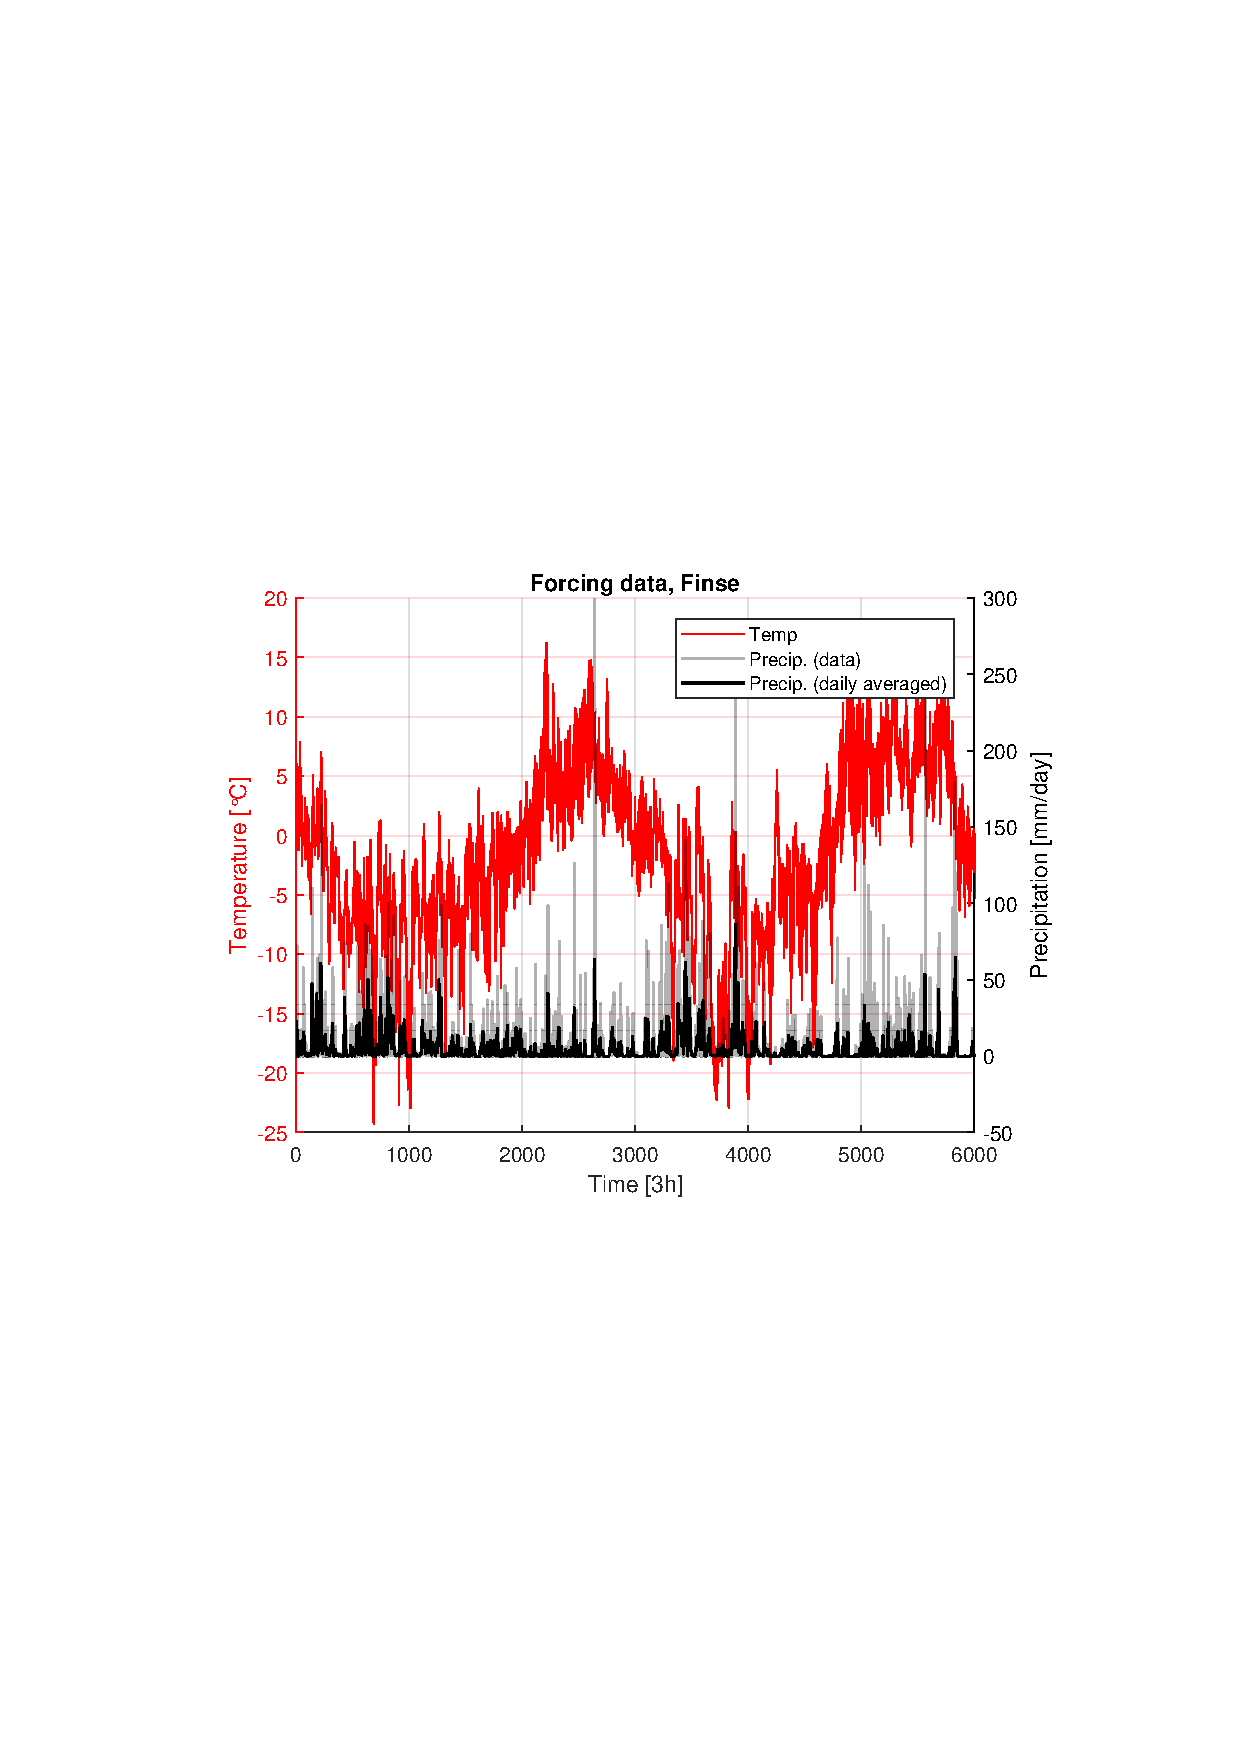
\includegraphics[width=0.5\textwidth]{figures/forcing_finse}
	\caption{Temperature (red) and precipitation(grey) data from forcing file. Daily mean values (black) printed for readability.}
	\label{fig:forcing}
\end{figure}

The precipitation output from the bucket model results in Figure(\ref{fig:precip}). Now the precipitation flattens once the ground temperature drops below zero. The step-like feature in the second winter arises because the precipitation value is kept at the last recorded value with temperature above zero degrees.

\begin{figure}[h]
	\centering 
	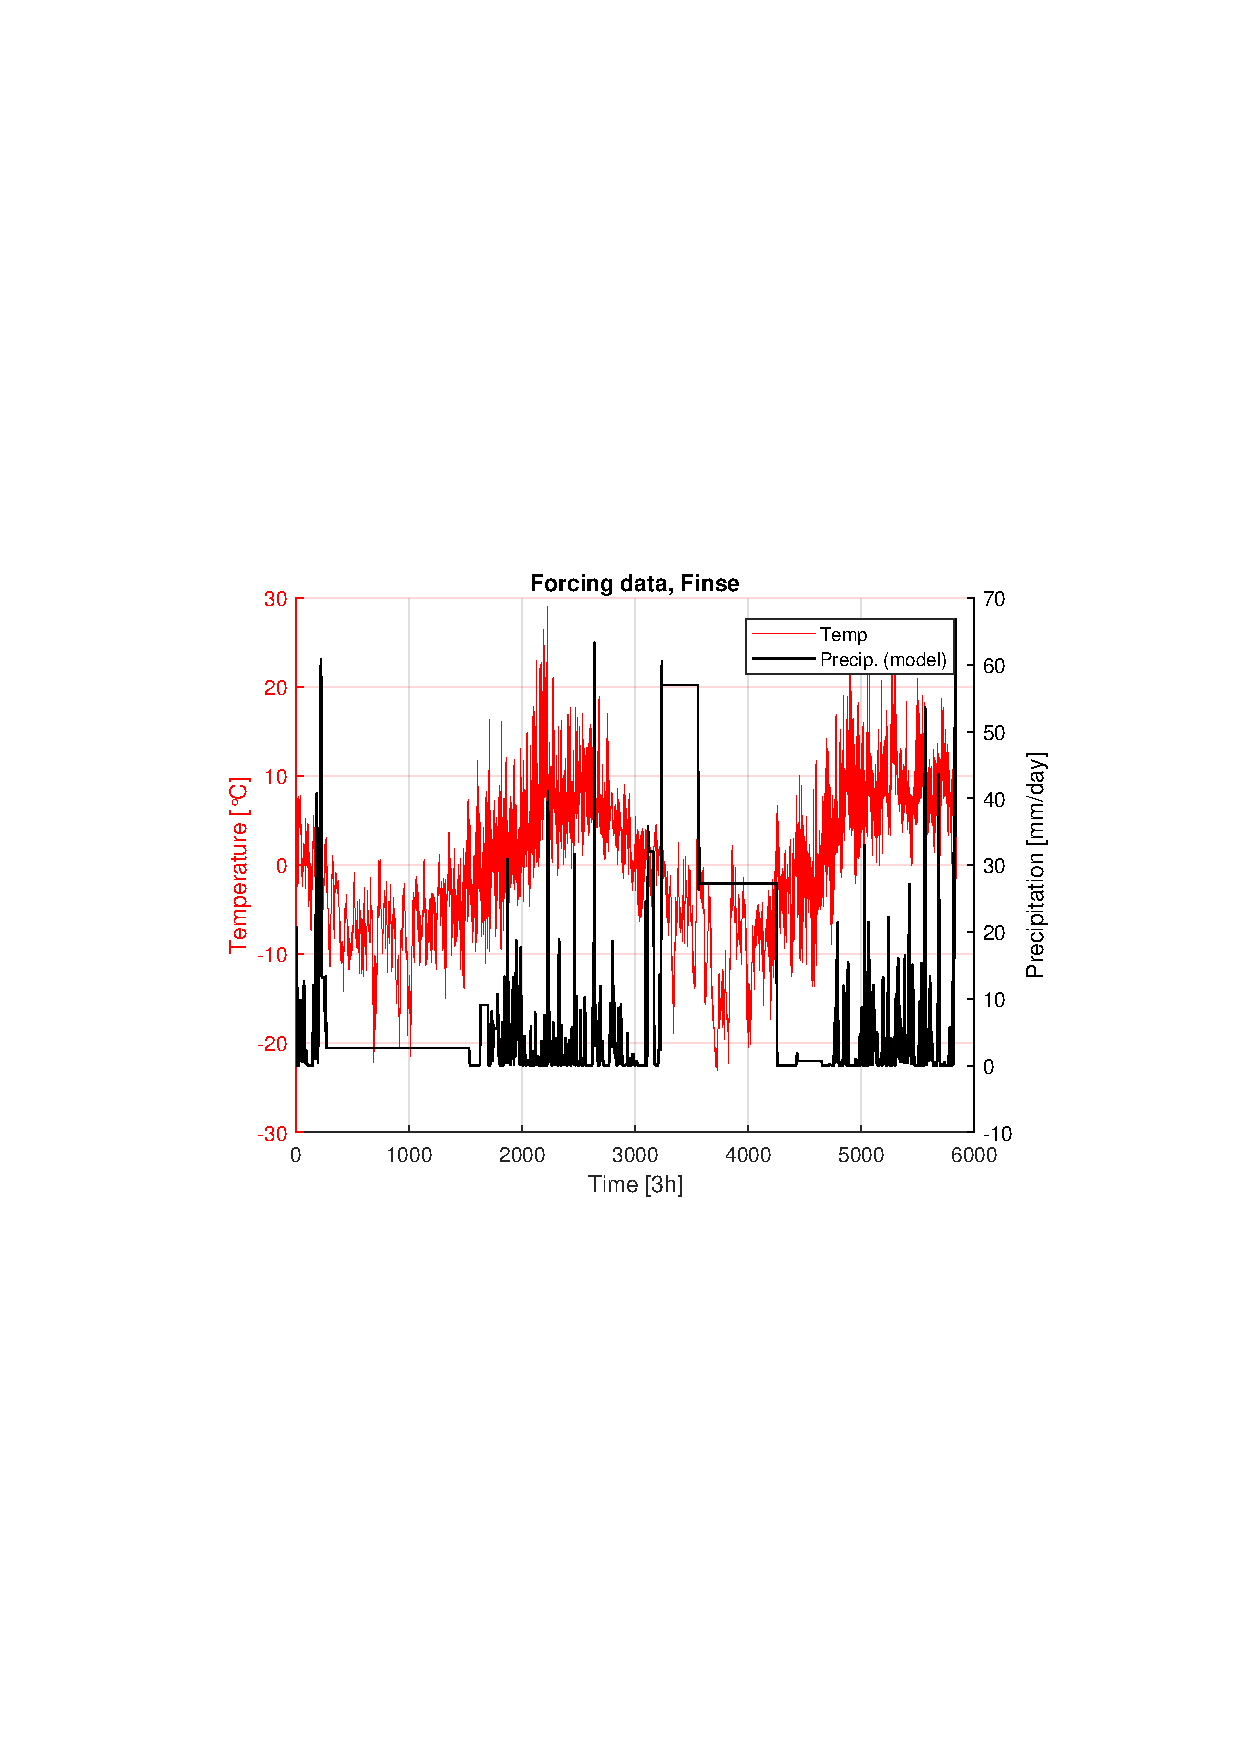
\includegraphics[width=0.5\textwidth]{figures/precip}
	\caption{Surface temperature (red) and precipitation(black) from the bucket model.}
	\label{fig:precip}
\end{figure}

Once we have established that the model is not allowing freezing, we look at how the soil deals with precipitation events. First, the bucket model is set with a constant initial water level of 0.1 meters. Figure(\ref{fig:bucket_fixed}) shows how the water level is rising after each precipitation event, but also how it drops if the precipitation ends. Now the flat part of the curves have two physical interpretations. Firstly, no precipitation occurs in these time slots as indicated by the grey line in the figure. Secondly,the bucket may have become full and is unable to store more water. Already in the first zero-precipitation window the shallowest bucket(0.2 meters)became full. The 0.4 meters deep bucket was close to full, but managed some more centimetres before getting filled in the first summer.
One interesting feature is that both the 0.8 meters and 1.0 meters buckets makes it though the entire summer without reaching their limits. \textbf{Some source on if this is usual or not?}. The 0.6 meter bucket reaches saturation sometime towards the end of the first summer. 

\begin{figure}[h]
	\centering 
	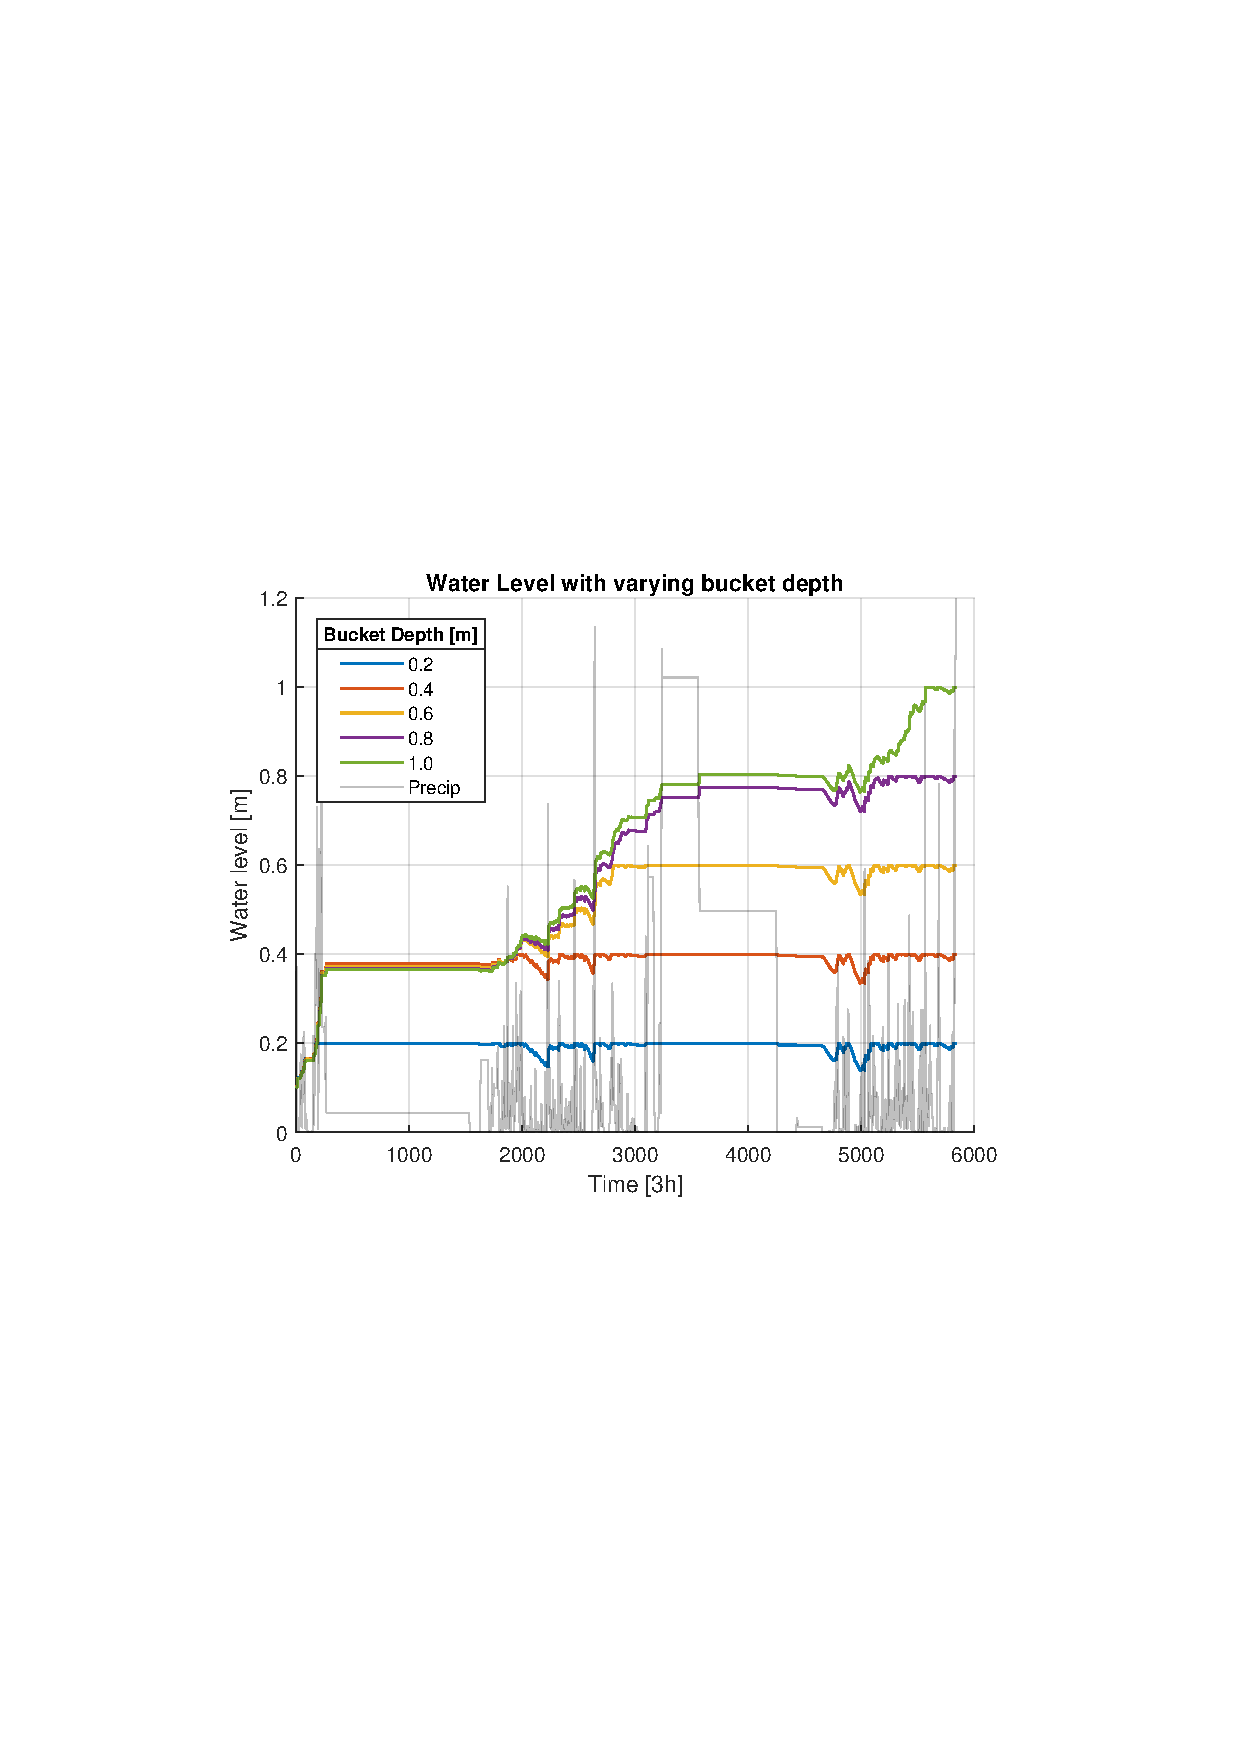
\includegraphics[width=0.5\textwidth]{figures/bucket_depth_fixed}
	\caption{Water level in soil dependent on the bucket depth with an fixed initial water level of 0.1 meters. Gray line is precipitation for reference.}
	\label{fig:bucket_fixed}
\end{figure}

Since all of the buckets eventually reaches saturation, surface runoff will occur as shown in Figure (\ref{fig:runoff}). The runoff values are relatively high compared to the precipitation values. This is expected since the soil layer in this case is thin. Each of the buckets experiences runoff where one deeper bucket also experiences runoff. Towards the end of the plot in Figure (\ref{fig:runoff}) it may look like only the deepest bucket experiences runoff, but since the deepest bucket experiences runoff at this point in time, all of the other buckets also experiences runoff. 

\begin{figure}[h]
	\centering 
	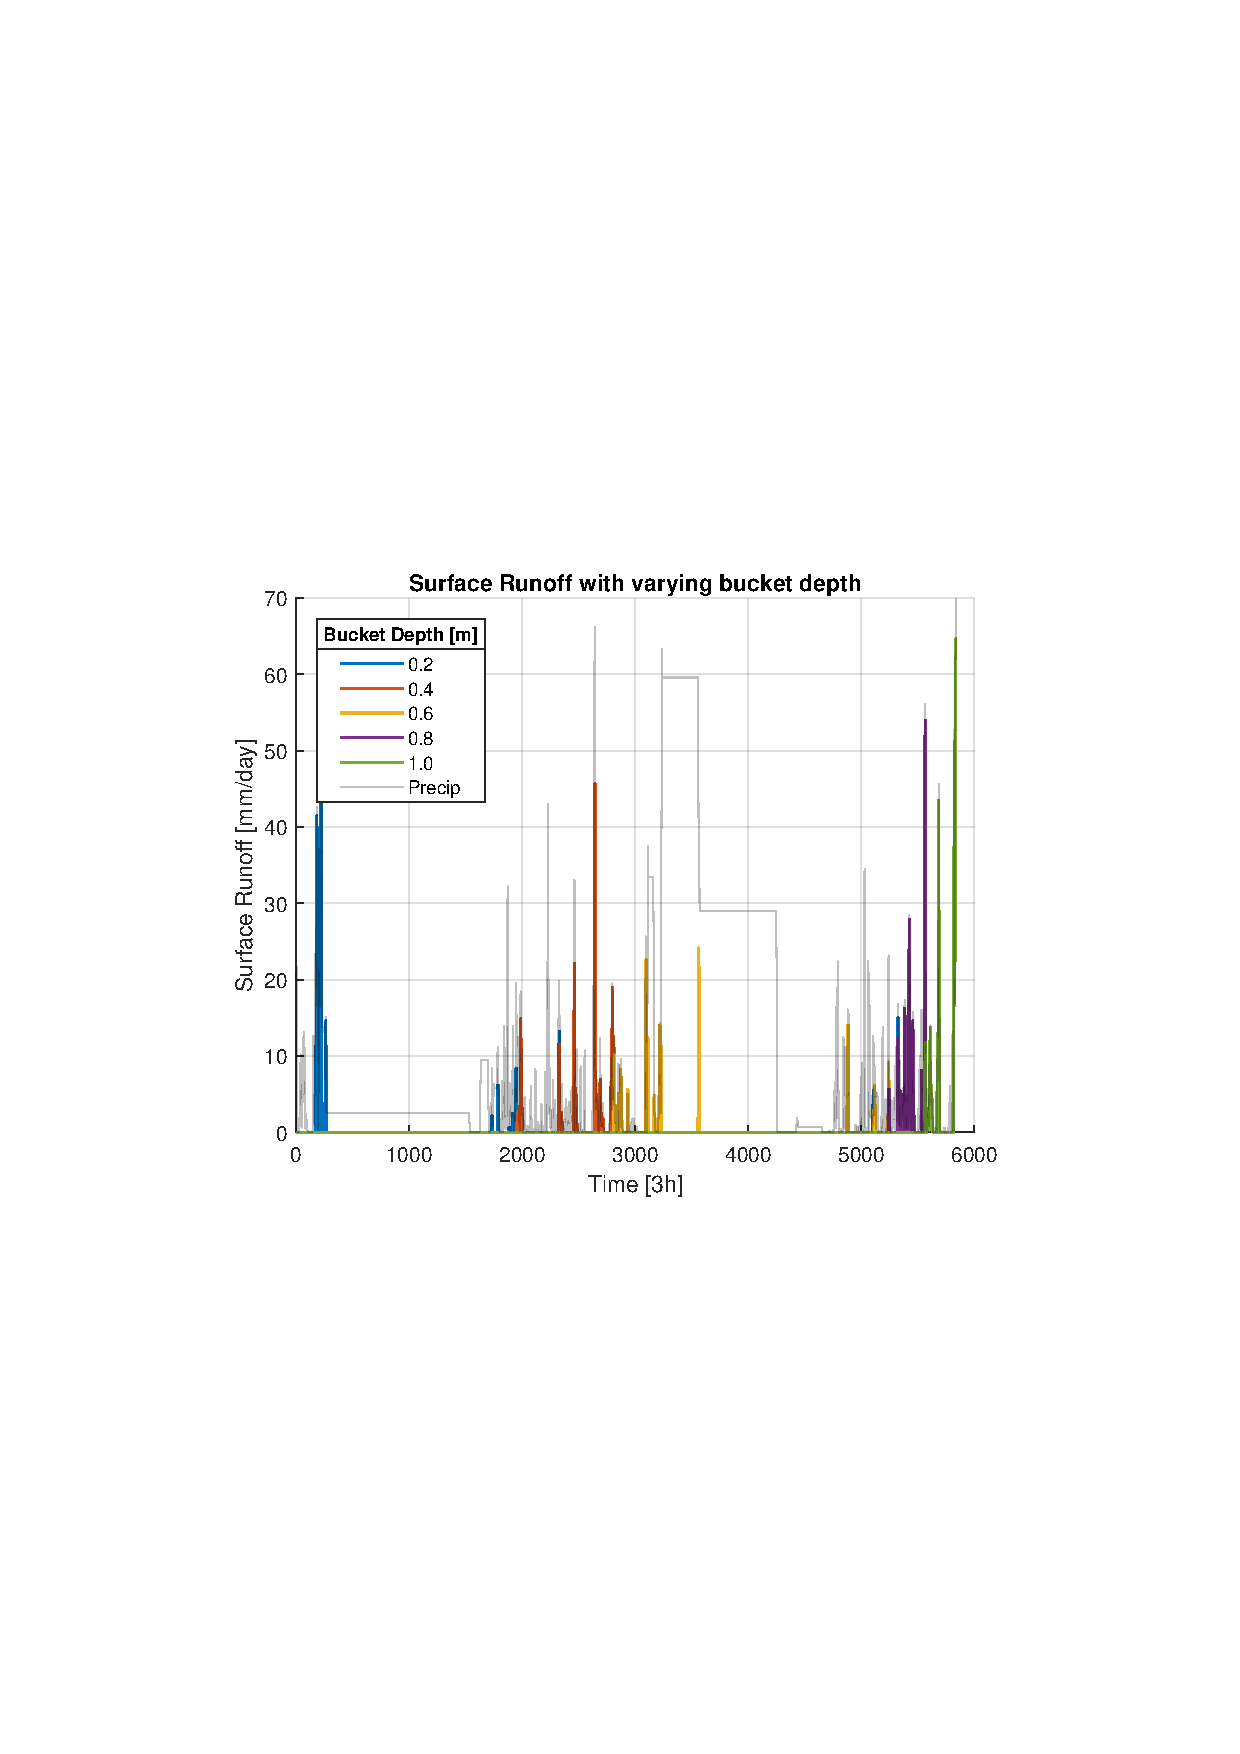
\includegraphics[width=0.5\textwidth]{figures/runoff}
	\caption{Surface runoff with varying bucket depth. Gray line is precipitation for reference.}
	\label{fig:runoff}
\end{figure} 

\section{Discussion}
The fact that the 0.6 meter bucket in  Figure(\ref{fig:bucket_fixed}) almost made it through the entire summer without getting saturated may indicate that there are some other important processes for removal of water at Finse in action. Evaporation may attribute to this. Resulting values for evaporation displayed in Figure (\ref{fig:evaporation}) reveals daily values for evaporation between 5 and 10 mm to be quite common.    
\begin{figure}[h]
	\centering 
	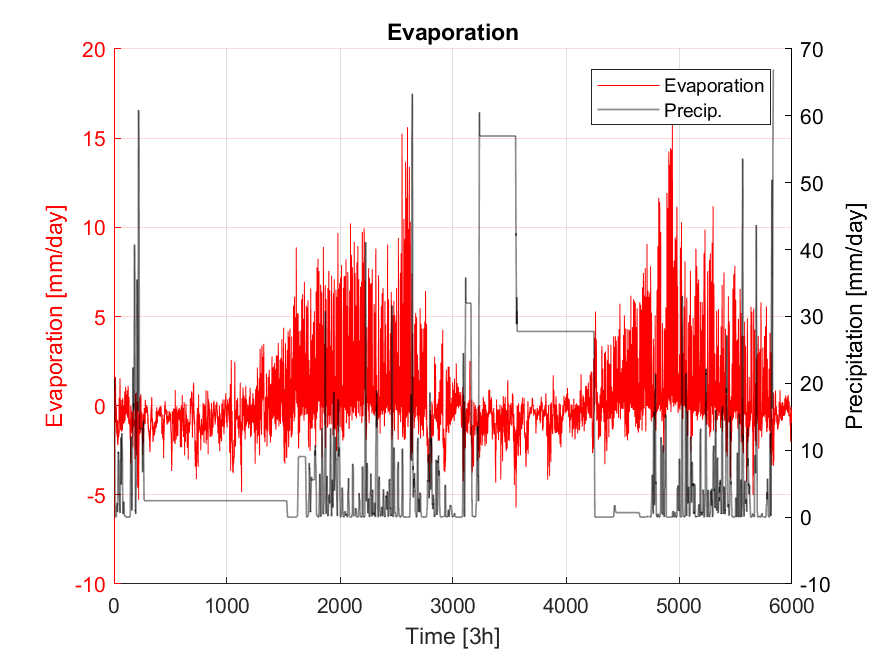
\includegraphics[width=0.5\textwidth]{figures/evaporation}
	\caption{Evaporation with varying bucket depth. Gray line is precipitation for reference.}
	\label{fig:evaporation}
\end{figure} 
\\
\textbf{vurder om du vil ke drainage constant til emre enn 1, vil si at det er realistisk med litt høyere verdi?}
\section{Future Work}
calculate how much runoff we have in percent from precipitation
caculate rates at with saturation increasesdecreases
\twocolumn
[
\begin{@twocolumnfalse}


\medskip

\begin{thebibliography}{9}

\bibitem{muller}
MÜller et al. 2017\\
\textit{AROME-MetCoOp: A Nordic Convective-Scale Operational
Weather Prediction Model}\\
URL: \url{https://doi.org/10.1175/WAF-D-16-0099.1}

\bibitem{dingman}
S. Lawrence Dingman \\
\textit{Physical Hydrology}\\
Third Edition \\
Waveland Press, 2015.\\

\bibitem{finse}
Webpage of Finse Alpine Research Ceenter\\
URL: \url{https://www.finse.uio.no/about/location/}\\
Visited 20th of April 2020

\bibitem{yr}
URL: \url{https://www.yr.no/nb/historikk/graf/1-111123/Norge/Vestland/Ulvik/Finse}


\end{thebibliography} 


\end{@twocolumnfalse}
\
]

\end{document}